\documentclass[../main.tex]{subfiles}
\graphicspath{{\subfix{../Figures/}}}
\begin{document}
    \begin{frame}{Why mixing is hard in hypergraphs?} 
        \begin{itemize}
        	\item Proving mixing in hypergraphs is harder because it is not possible to define an equivalent discrete diffusion process as a random walk.
        	\item The Laplacian operator $\mathcal{L}$ s.t. $\frac{d \bold{p}_t}{d t} = -\mathcal{L}(D^{-1}\bold{p}_t)$ can be defined for $B_e$ the convex hull of $\{\chi_v-\chi_u : u,v\in e\}$ \cite{continuous_laplacian_hypergraph} as:
	        	\begin{columns}
	        		\column{0.8\textwidth}
	        		\begin{block}{Laplacian for hypergraphs}
	        			$ \mathcal{L}(\bold{x}) = \{\sum_{e\in E} w_e \bold{b}_e\bold{b}_e^T \bold{x} \mid \bold{b}_e = \argmax_{\bold{b}\in B_e} \bold{x}^T\bold{b} \}$
	        		\end{block}
	        	\end{columns}
	        \begin{columns}
	        	\column{0.8\textwidth}
	        	\raisebox{-1.1\height}{	        	
			        \hspace{3cm}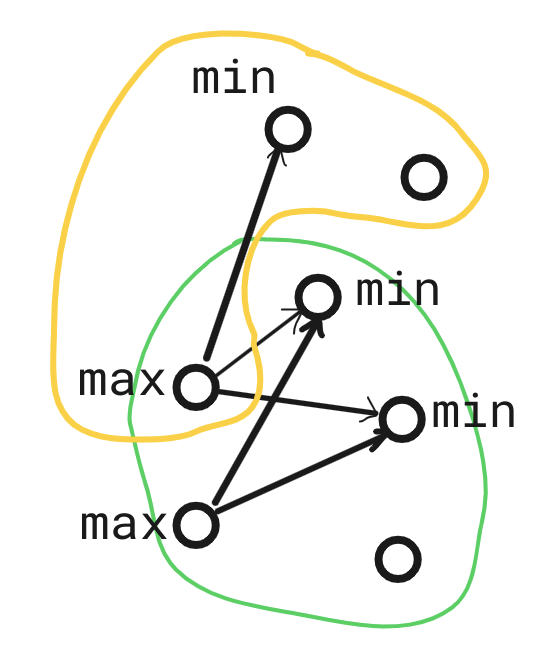
\includegraphics[width=0.3\textwidth]{hypergraph_laplacian_operator}}
	        \end{columns}
        \end{itemize}
    \end{frame}
		
	\begin{frame}{Discrete diffusion process}
		\begin{itemize}
			\item Idea: turn the hypergraph laplacian into a matrix by solving ties \textit{arbitrarily}. 
			\item Question: is this simple resolution of ties enough in order to obtain a diffusion process with good mixing properties?
		\end{itemize}
	\end{frame}

	\begin{frame}{Discrete diffusion process}
		\begin{itemize}
			\item We collapse the hypergraph $H$ into a multigraph $G_t$ collapsing every hyperedge $e$ into $(v_{\text{max}}^t(e), v_{\text{min}}^t(e))$
				\begin{columns}
					\column{0.8\textwidth}
					\begin{block}{$v_{\text{max}}^t(e)/ v_{\text{min}}^t(e)$}
						$v_{\text{max}}^t(e) = u\in e : \argmax/\argmin_{u\in e} \frac{p_t(u)}{d(u)}$
					\end{block}
				\end{columns}
			\begin{columns}
				\hspace{1cm}\column{0.5\textwidth}
					Hypergraph $H$
					\hspace{2cm}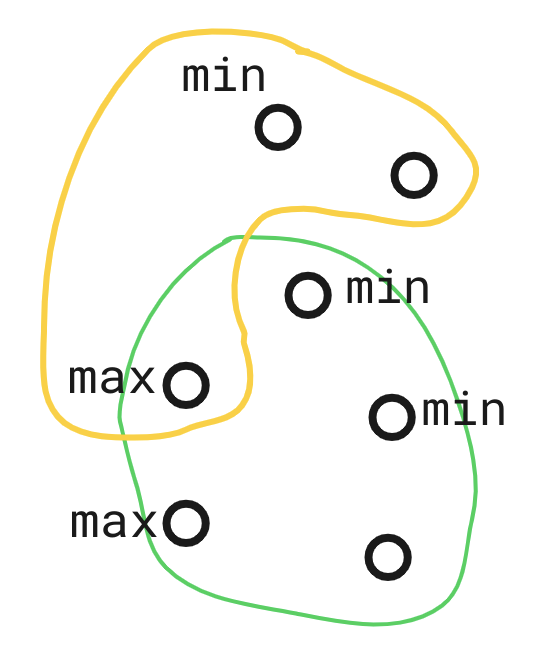
\includegraphics[width=.5\textwidth]{collapsed_hypergraph}
				\column{0.5\textwidth}
					Collapsed multigraph $G_t$
				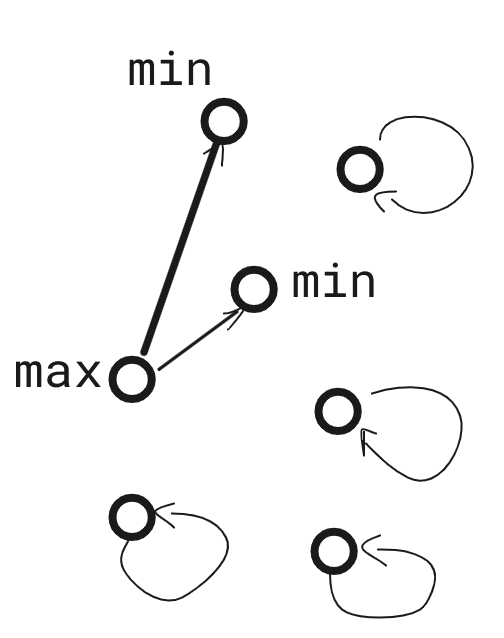
\includegraphics[width=.5\textwidth]{collapsed_multigraph}
			\end{columns}
		\end{itemize}
	\end{frame}

	\begin{frame}{Discrete diffusion process}
		We want to use the Lovasz Simonovits recursive upper bound in order to prove mixing of this diffusion process.
		\begin{block}{LS recursive upper bound for $dt\leq \frac{1}{2}$}
			$I_{t+dt}(k) \leq (1-2dt)I_t(k) + dt(I_t(k - \hat{k}\hat{\phi}) + I_t(k + \hat{k}\hat{\phi})$
		\end{block}
		So we need the cut $S_j(p_{t+dt})$ to have conductance $\phi(S_j(p_{t+dt})) = \hat{\phi}$ in both the collapsed multigraphs $G_t$ and $G_{t+dt}$.
	\end{frame}
	\begin{frame}{Discrete diffusion process}
		Every hyperedge crossing the cut $S_j(p_{t+dt})$ is collapsed in the multigraph $G_{t+dt}$ in such a way that it also crosses the cut. But, this is not necessarily true for the graph $G_t$.
		\begin{columns}
			\column{0.33\textwidth}
				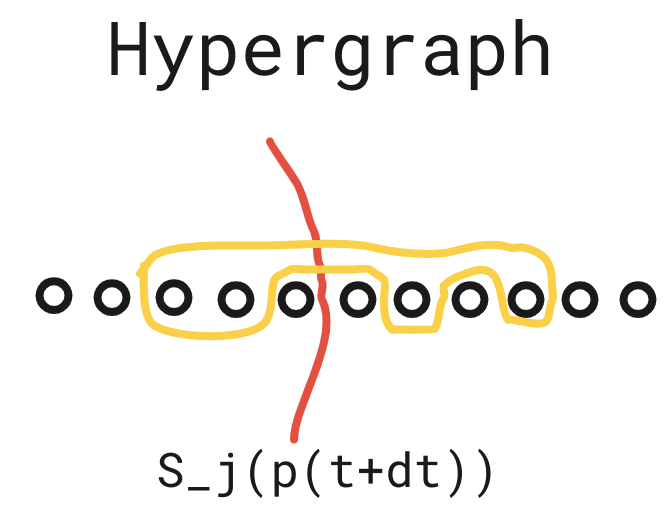
\includegraphics[width=0.8\textwidth]{hyperedge_crossing_sweep_cut_t_dt}
			\column{0.33\textwidth}
				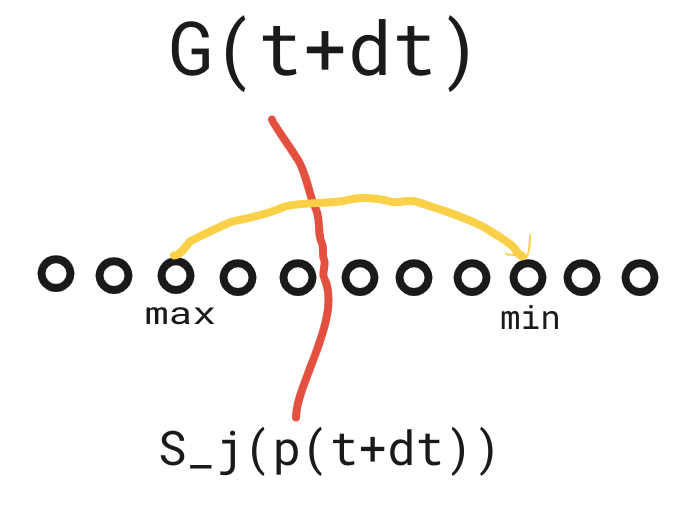
\includegraphics[width=0.8\textwidth]{collapsed_edge_crossing_sweep_cut_t_dt}
			\column{0.33\textwidth}
			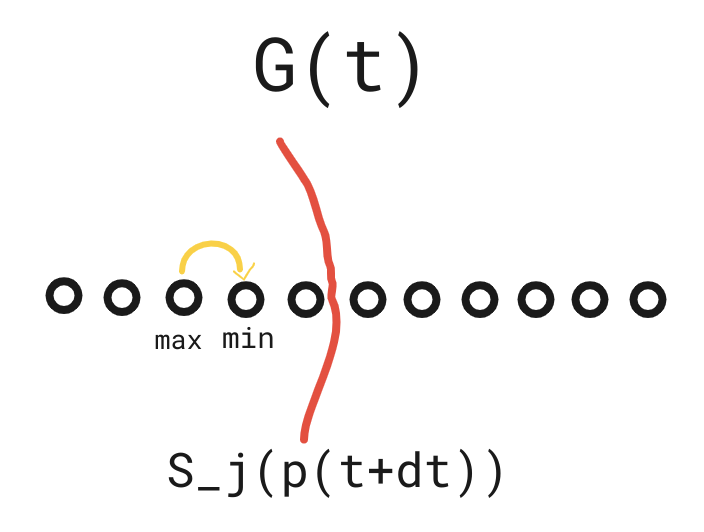
\includegraphics[width=0.8\textwidth]{collapsed_edge_crossing_sweep_cut_t}
		\end{columns}
		\begin{columns}
			\column{0.5\textwidth}
			We can add another edge to $G_t$ which is certainly crossing the cut.
			\column{0.5\textwidth}
			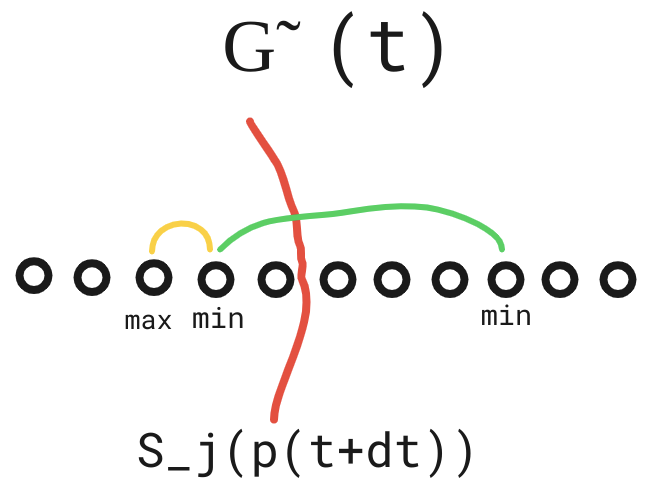
\includegraphics[width=0.5\textwidth]{collapsed_edge_crossing_sweep_cut_t_tilde}
		\end{columns}
		
	\end{frame}

	\begin{frame}{Discrete diffusion process}
		The proof of the mixing result goes like this:
		\begin{itemize}
				\item First, prove that the LS-curve $\tilde{I}_t$ is smaller than $I_t$. 
				\begin{lemma}
					\label{lemma:ls_curve_smaller_ls_curve_tilde}
					$\forall t$, 
					$I_{t+dt}(k) \leq \tilde{I}_{t+dt}(k)$
				\end{lemma} 
			\item Then, take advantage of the known conductance of the sweep cuts in $\tilde{G}_t$ to prove
				\begin{lemma}
					\label{lemma:recursive_LS_lower_bound}
					$\tilde{I}_{t+dt}(k) \leq (1-2dt) I_t(k) + 2dt (I_t(k-\hat{\phi} \hat{k}) + I_t(k + \hat{\phi}\hat{k}))$
				\end{lemma}
			\item Which allows us to claim
				\begin{lemma}
					\label{lemma:mixing_result} 
					$I_t(k) - \pi(S_j(\bold{p}_t)) \leq \sqrt{\frac{k}{d(v_0)}} e^{-t \hat{\phi}^2}$
				\end{lemma}
		\end{itemize}
	\end{frame}

%	\begin{frame}{Proof of Lemma \ref{lemma:ls_curve_smaller_ls_curve_tilde}}
%		\begin{block}{Lemma \ref{lemma:ls_curve_smaller_ls_curve_tilde}}
%			$\forall k\in[0,\text{vol}(H)], \forall t, I_{t+dt}(k) \leq \tilde{I}_{t+dt}(k)$
%		\end{block}
%		\begin{proof}
%			The idea is that $\forall u\in S_j(\bold{p}_{t+dt})$, the new edges $(u,v)$ added to $\tilde{G}_t$ are such that $v$ has higher $\frac{p_t(v)}{d(v)}$ value than $\frac{p_t(u)}{d(u)}$. This ensures that the probability at time $t+dt$ on $u\in S_j(\bold{p}_{t+dt})$ is higher, and hence $\tilde{I}_{t+dt}(k) \geq I_{t+dt}(k)$.
%		\end{proof}
%	\end{frame}

%	\begin{frame}{Proof of Lemma \ref{lemma:recursive_LS_lower_bound}}
%		\begin{block}{Lemma \ref{lemma:recursive_LS_lower_bound}}
%			$\tilde{I}_{t+dt}(k)\leq (1-2dt)I_t(k) + dt(I_t(k-\hat{\phi}\hat{k}) + I_t(k+\hat{\phi}\hat{k}))$
%		\end{block}
%		\begin{proof}
%			\begin{itemize}
%				\item In order to prove Lemma \ref{lemma:recursive_LS_lower_bound} you split edges (and self loops) in groups:
%				\begin{itemize}
%					\item $W_1 = \{u,v: u,v\in \bar{S}_j(\bold{p}_{t+dt})\}$ 
%					\item $W_2 = \{u,v: u\in S_j(\bold{p}_{t+dt}) \text{ and } v\in S_j(\bold{p}_{t+dt})\}$
%					\item $W_3 = \{(u,u) : \text{vol}(W_3) = dt\cdot\text{vol}(S_j(\bold{p}_{t+dt}))\}$
%					\item $W_4 = \{(u,u) : \text{vol}(W_4) = (1-2dt)\text{vol}(S_j(\bold{p}_{t+dt}))\}$
%				\end{itemize}
%				\item Then you prove the three bounds:
%					\begin{itemize}
%						\item $\tilde{\bold{p}}_{t+dt}(W_1) \leq dt \cdot I_t(\text{vol}(S_j(\bold{p}_{t+dt})) - \frac{\text{vol}(W_2)}{dt})$
%						\item $\tilde{\bold{p}}_{t+dt}(W_2\cup W_3)\leq dt\cdot I_t(\text{vol}(S_j(\bold{p}_{t+dt})) + \frac{\text{vol}(W_2)}{dt})$
%						\item $\tilde{\bold{p}}_{t+dt}(W_4) \leq (1-2dt) I_t(\text{vol}(W_4))$
%					\end{itemize}
%				\item and conclude by noticing that $I_t$ is concave, and $\frac{\text{vol}(W_2)}{dt} \geq \hat{\phi}\hat{k}$.
%			\end{itemize}
%		\end{proof}
%	\end{frame}
%
%	\begin{frame}{Proof of Lemma \ref{lemma:mixing_result}}
%		\begin{block}{Lemma \ref{lemma:mixing_result}}
%			$I_t(k) - \pi(S_j(\bold{p}_{t})) \leq \sqrt{\hat{k}} e^{-\frac{t\hat{\phi}^2}{4}}$
%		\end{block}
%		\begin{proof}
%			First, we define support function $$R_t(k) = \begin{cases} \sqrt{k} & t=0 \\ (1-2dt)R_{t-dt}(k) + dt(R_{t-dt}(k-\hat{\phi}\hat{k}) + R_{t-dt}(k+\hat{\phi}\hat{k})) & t>0
%			\end{cases}$$
%			And then prove $I_t(k)\leq R_t(k)$ by induction on $t$. Finally, it is possible to prove $R_t(k) \leq \sqrt{k}e^{-\frac{t\hat{\phi}^2}{4}}$ by induction on $t$, using Taylor expansion $\sqrt{1-\hat{\phi}}+\sqrt{1+\hat{\phi}} \leq (1-\frac{\hat{\phi}^2}{8}) \leq e^{-\frac{\hat{\phi}^2}{8}}$
%		\end{proof}
%	\end{frame}
\end{document}